\documentclass[a4paper,10pt]{book}
\usepackage[utf8]{inputenc}
\usepackage{listings}
\usepackage{textcomp}
\usepackage{color}
\usepackage{hyperref}
\usepackage{graphicx}

% This document (including sub files) is made available under 
% Creative Commons Attribution-ShareAlike 4.0 International (CC BY-SA 4.0)
% Original document by Joel Fenwick - 2016
% Contributions by Joel Fenwick are copyright by The University of Queensland
% Additional authors added for non-trivial contributions


% Design principles:
%  * this is not intended to be a textbook - it is supposed to support lectures or other reasources
%  * it is intended to be usable (if not optimal) as both a reference and as a tutorial
%  * forward concept references are to be avoided.  If something is presented as an example which
%    readers are supposed to learn from, then they should be able to understand everything in that example.
%    That is not to say concept explanations can't be iterated/elaborated on later
%  * System/environment specific details should be separated into their own files so they can be disabled/switched out.
%  * Except for small fragments, hypreref link to programs so they can be placed elsewhere in the document/floated.
%  * Only use widely available LateX packages --- distributed with or autodownload for most major LaTeX distributions.
%    Think you need to add a class or package to this repo, please think again.
%  * Content is to be restricted to standard-C99


\newcommand{\todo}[1]{\textbf{#1}}
\lstset{basicstyle=\ttfamily,
	columns=flexible, % To convince it to do the right thing with quotes
	language=C,
	upquote=true,
	showstringspaces=false,
	escapechar=~,
	keywordstyle=\color[rgb]{0,0,1},
	commentstyle=\color[rgb]{0.133,0.545,0.133},
	stringstyle=\color[rgb]{0.627,0.126,0.941}
}
\lstnewenvironment{codeblock}{\lstset{
		numbers=left,
		frame=l}}{}
\lstnewenvironment{codeinline}{\lstset{
		frame=none,
		numbers=none}}{}
	
		
\begin{document}

\title{A C tutorial/refresher}
\author{Joel Fenwick (editor)}
\addcontentsline{toc}{section}{Cover}
\maketitle

\tableofcontents
\addcontentsline{toc}{section}{Contents}
\lstset{language=C}

\chapter{Commandline Linux environment --- gcc}

The following assumes that you have access to a Linux/Posix/BSD commandline.
This could either be a local terminal window on operating systems which support it or via an SSH program such as Putty.
We will assume you are using the \texttt{bash} shell and the \texttt{gcc} C compiler.

\section{Creating source files}
C source files can be created and edited using any plain text editor\footnote{Some tools (such as MacOS's TextEdit) can save formatting or not. Make sure you are using text only.} (eg: \texttt{nano} or \texttt{vim}).
Be aware that different operating systems have different ideas about what the end of a line looks like.
For example, compiling a file on Linux which has Windows line endings in it will lead to compile errors.
With this in mind, try to edit on the same platform you will be compiling on (or failing that, use a tool which respects the target
platform's line endings\footnote{For example, Notepad++ can be set to act in this way.}.

Some systems have case-sensitive filenames and some are case-insensitive (eg: \texttt{bob.c} is considered to be the same file as \texttt{Bob.C}).
Regardless of your home system, you should try to use consistent cases.
For \texttt{gcc}, C source files must end in \texttt{.c} (lower case) or later on \texttt{.h}.

Put the following in a file called \texttt{test.c}:
\begin{lstlisting}
int main()
{
    return 5
}
\end{lstlisting}

Then compile it with the command:
\begin{verbatim}
gcc test.c 
\end{verbatim}
which will produce a message like:
\begin{verbatim}
test.c: In function ‘main’:
test.c:4:1: error: expected ‘;’ before ‘}’ token
 }
 ^
\end{verbatim}

Now type:
\begin{verbatim}
echo $? 
\end{verbatim}

This asks the shell to tell you what happened with the previous command (its ``exit status'').
By tradition, anything other than $0$ indicates some form of error.
In this case, the compiler failed and \verb!$?! reflects that.
Now edit \texttt{test.c} to add a semicolon after the $5$, then recompile.
You should not see any messages.

Look in the current directory, and you should see a new file called \texttt{a.out}.
This is the default name for programs made with \texttt{gcc}. The name can be changed
by using the ``-o'' option:

\begin{verbatim}
gcc test.c -o test
\end{verbatim}
This would produce an output file named \texttt{test}.
\\
Execute your program with:
\begin{verbatim}
./a.out 
\end{verbatim}
and check that the exit status was $5$ as exepected. When a program returns from main its ``exit status'' is the value returned.

Depending on your requirements, you may need to comply with some particular version of the C language standard.
Adding one of the following to your compile line will do this.

\begin{tabular}{c|c}
-ansi & C89/C90 \\
-std=c99 & C 99 \\
-std=gnu99 & C99 with some gnu extras\\
\end{tabular}


\section{Linking and other compile options}
\texttt{gcc test.c} actually performs a number of phases including compiling and linking.
The distinction between these is more important when a program's source consists of multiple 
files.
\begin{verbatim}
gcc -c file1.c
gcc -c file2.c
gcc -c file3.c
\end{verbatim}
Would compile each of the files (and check them for correctness).
Following that:
\begin{verbatim}
gcc file1.o file2.o file3.o 
\end{verbatim}
would ``link'' i.e. combine the pieces together and check for consistency and completeness.

Adding \texttt{-Wall} and/or \texttt{-pedantic} will cause \texttt{gcc} to report more potential problems.
\emph{This is a good thing.}

\section{Other notes}
It may seem obvious, but do not ignore error or warning messages.

You can save error messages by adding \verb|2>errfilename| to the end of a command.
For example:
\begin{verbatim}
gcc myfile.c 2>errors.log
\end{verbatim}






\chapter{First program}
\lstset{numbers=left, showstringspaces=false, frame=l}

\todo{Need to have concepts this section assumes:    strings and arrays.}


Compile and run the following:
\begin{lstlisting}
#include <stdio.h>

int main(int argc, char** argv) {
    printf("It begins\n");
    return 0;
}
\end{lstlisting}

\begin{itemize}
 \item[1] \lstinline!#include! is a ``preprocessor directive''\footnote{as opposed to a C statement or declaration} which tells gcc to 
 consult another file before going any further.  If you remove this line, you will see that \texttt{printf} becomes a problem.
 This is because the \texttt{stdio.h} file is what tells \texttt{gcc} about the \texttt{printf} function.
 
 The $<>$ around the \texttt{stdio.h} indicate that it is a system include rather than a header we created ourselves\footnote{
 More accurately, $<>$ indicate which paths the compiler should look for the file in.}.
 For our own headers, put the filename in double quotes.
 
 \item[3] begins a function definition\footnote{A definition tells the compiler both that the function exists(called declaration), and what the function does}.
 All standard C programs must have a function called \texttt{main}.
 Unless your system has special requirements, you should use the signature\footnote{A function's signature gives the function's name, its return type and the type and order of parameters.} shown here.
 We have not discussed types yet (we'll look at types in See Item~???) but for now, \texttt{int} is an 
 integer\footnote{A whole number, either positive or negative} while \texttt{char} on its own represents a character.
 The first \texttt{int} means that our \texttt{main} function returns an int.
 The parts in parentheses are the parameters for the function.
 The first one is an integer and the second one has something to do with characters.
 Without explaining why now, the second parameter is an array of strings.
 Note that this program doesn't actually make use of the parameters it is passed.
 
 \item[4] This is a function call. It has the name of a function \texttt{printf} followed by arguments in parentheses.
 Text in double quotes represents a string. 
 So this line passes a string to the \texttt{printf} function.
 
 \item[5] indicates which value the function returns/sends back to its caller.
 For main, the return value is sent back to the operating system as the program's exit status.
\end{itemize}



\chapter{Simple output and Command Line arguments}


Compile and run the following:
\begin{lstlisting}
#include <stdio.h>

int main(int argc, char** argv) {
    printf("Going to print some things %s%s%s\n");
    return 0;
}
\end{lstlisting}

Although you \emph{can} just print strings directly with printf, it isn't necessarily a good idea (as shown above)\footnote{\texttt{puts()} is probably a better option}.
To understand why, we need to look at how \texttt{printf} deals with variables.
Replace Line~$4$ with \lstinline!printf("%s\n", "Going to print some things %s%s%s ");!

The first parameter of \texttt{printf}, describes what is to be printed, any sequence starting with \% is called a placeholder and will be replaced with something else when the output is done.
Characters after the \% indicate what type of thing is to be printed (and possibly how it is to be formatted).
So \%s in the first argument tells \texttt{printf} that it should look at the next argument along, interpret it as a string and print it.
If there aren't enough arguments, or the argument is the wrong type, unexpected things may occur.

To print an integer instead of a string, use the \%d placeholder.
For example: \lstinline!printf("%d + %d = %d\n", 5, 7, 12);!
You can use any mixture of placeholders and normal characters in the \emph{format string} that you like.
To print a \% symbol, use \%\%.


Compile the following:
\begin{lstlisting}
#include <stdio.h>

int main(int argc, char** argv) {
    printf("There were %d arguments given to the program %s\n",
      argc, argv[0]);
    return 0;
}
\end{lstlisting}
Lines~4 and 5 show that you can break lines to improve layout and readability.
Try running the program with a variety of command line arguments.
You will see that \texttt{argv[0]}, contains the name of the program (\texttt{argv} stands for ``argument values") and that \texttt{argc} gives the ``argument count'' --- how many there were).
Since the argv always has at least one thing in it, argc$\geq 1$ and accessing argv[0] should always be safe.
But change the program to print argv[200] and see what happens.


By using a conditional statement, we can safely print more if it is available.
\begin{lstlisting}
#include <stdio.h>

int main(int argc, char** argv) {
    printf("0: %s\n", argv[0]);
    if (argc > 1) {
      printf("1: %s\n", argv[1]);    
    }
    if (argc > 2) {
      printf("2: %s\n", argv[2])
    }
    return 0;
}
\end{lstlisting}
Some type of loop would be a better way to deal with this, so let's do that now.

\section{Loops}
A loop consists of the following parts (some of which may be empty):
\begin{itemize}
 \item [Setup] --- happens once (before the loop starts).
 \item [Test]  --- should the loop repeat or stop now?
 \item [Body]  --- what the loop is supposed to do each time.
 \item [Update] --- happens after the body runs each time.
\end{itemize}

So to display command line arguments:
\begin{itemize}
 \item [Setup] --- set a counter variable (\texttt{i}) to 0.
 \item [Test]  --- is \texttt{i} less than \texttt{argc}
 \item [Body]  --- print the argument
 \item [Update] --- increase \texttt{i}
\end{itemize}

C has three types of loop structure:

The \emph{for} loop
\begin{lstlisting}
for (Setup ; Test ; Update) {
    Body
}
\end{lstlisting}

The \emph{while} loop
\begin{lstlisting}
Setup
while (Test) {
    Body
    Update
}
\end{lstlisting}

and the \emph{do-while} loop
\begin{lstlisting}
Setup
do {
    Body
    Update
} while(Test);
\end{lstlisting}

The \emph{do-while} loop differs from the \emph{while} loop by always running the Body and Update once before the Test is performed and the loop loops.

So we could do this:
\begin{lstlisting}
#include <stdio.h>

int main(int argc, char** argv) {
    for (int i = 0; i < argc; i = i + 1) {
        printf("%d: %s\n", i, argv[i]);
    }
    return 0;
}
\end{lstlisting}

As an exercise, rewrite the above to use \texttt{while} and then to use \texttt{do-while}.


\chapter{Operators and expressions}

%Until now, I've avoided putting (non-atom) expressions into calls.

In most cases in C, where you write literal values, you can write expressions\footnote{More information:
there are some things which need to be known at \emph{compile time} rather than \emph{run time}.
The most obvious cases of this are \emph{case labels} and array sizes in ANSI-C.}.
An expression is a fragment of code which can be ``evaluated'' --- that is, they can be processed to get a value.
For example:
\texttt{3+4} is an expression which gives the value $7$ when evaluated.
In fact, literal values are also expressions (they evaluate to the value as written).

\section{Arithmetic operators}

The operators $+$ and $-$ work as you would expect.
Division is written with $/$ and multiplication as $*$.

The \% operator (known as ``modulo'') returns the remainder of its arguments;
\texttt{a\%b} returns the remainder when \texttt{a} is divided by \texttt{b}.
For example: $7\%3$ is $1$   and $23\%5$ is $3$.


\subsection{Precedence}
When an expression involves more than one type of operator, the issue of precedence comes up.
That is, some operators are evaluated before others --- this is independent of the order the operators are written in.
The rules for $+,-,*,/$ are the same as for normal arithmetic.

You can look up the precedence for operators, but you can also test them.
For example, $+$ and $*$ could be compared like this:
(Enter and run the following)
\begin{lstlisting}
#include <stdio.h>

int main(int argc, char** argv) {
    printf("%d %d %d\n", (2 + 3 * 7), ((2 + 3) * 7),
            (2 + (3 * 7))); // Continues from prev line.
    if ((2 + 3 * 7) == ((2 + 3) * 7)) {
        printf("+ is evaluated first\n");    
    } else if ((2 + 3 * 7)==(2 + (3 * 7))) {
        printf("* is evaluated first\n");
    } else {
        printf("Something has gone horribly wrong\n");
    }
    return 0;
}
\end{lstlisting} 

\noindent Exercise: Modify the program above to test relative precedence of \texttt{+} and \texttt{\%}.

\subsection{Simple Types}
All of C's simple types are numeric in some way.
This includes types which have other purposes (\texttt{char} and \texttt{bool}).

Numeric types can be classified in a number of ways:
\begin{itemize}
 \item Integer vs Floating point --- \texttt{bool\footnote{\texttt{stdbool.h} must be included to use \texttt{bool} (and \texttt{true} and \texttt{false}).}, char, int} are integer types while \texttt{float} and \texttt{double} are floating point types.
Arithmetic operators which act on integers \emph{will evaluate to an integer result} so for example, \texttt{5/2} is \texttt{2}, not \texttt{2.5}.
Do not make this mistake:
\texttt{float f=2/3;}
\texttt{f} will contain $0$ not $0.66$.
This is because storing a value in a variable does not influence the way the expression is evaluated.

If an expression contains a mixture of types, its arguments will be converted to the most general type.
For example:
\texttt{2/3.0} will give a floating point result because one of its arguments is floating point\footnote{Somewhat confusingly, the default floating point type in C is \texttt{double} not \texttt{float}.}.
You could also achieve this with a \emph{cast}: \texttt{2/(float)3} or multiplication \texttt{(1.0*2)/3}.

 \item Signed vs Unsigned --- integer types can be restricted to store only positive values\footnote{and therefore store higher maximum values using the same number of bits because the sign bit can be used for value storage.}
 For example: \texttt{unsigned int}, \texttt{unsigned char}\footnote{\texttt{int} defaults to \texttt{signed int} but if you care whether your \texttt{char}s are signed or unsigned, it is better to be explicit.}
 
 \item size --- types can be modified to indicate how much memory they take\footnote{In C, these modifications are not absolutely defined in the standard.}. 
 Types which take more memory can store a larger range of values.
 For example:  \texttt{short int} and \texttt{long int} are smaller and larger than normal \texttt{int}s respectively.
 These can be combined with \texttt{signed} and \texttt{unsigned}.
\end{itemize}
There are other type modifiers but we'll keep this simple and standard\footnote{For example: \texttt{long long int}  and \texttt{quad double} are non-standard types.}.


To output other types with \texttt{printf}, different placeholders are required:
\begin{itemize}
 \item [\%e \%f \%g] --- all of these will output a \texttt{float} \emph{or} \texttt{double} but they format it in different ways.
 \item [\%c] --- prints a char (as a character rather than as a number).
 \item [\%hd] --- prints a \texttt{short int}.
 \item [\%ld] --- prints a \texttt{long int}.
 \item [\%u]  --- prints an \texttt{unsigned int}.
\end{itemize}
Consult documentation for other combinations.

\section{Bit operators}

These operators act on the individual bits in the value.

\begin{itemize}
 \item \lstinline|a&b| --- bitwise \emph{and} of the two values.
 \item \lstinline:a|b: --- bitwise \emph{or} of the two values.
 \item \lstinline|a^b| --- bitwise \emph{exclusive or} of the two values.
 \item \lstinline|a<<b| --- left shift \texttt{a} by \texttt{b} bits.
 \item \lstinline|a>>b| --- right shift \texttt{a} by \texttt{b} bits.
 \item \lstinline|~a| --- one's complement of \texttt{a}.
\end{itemize}

\section{Relational operators}

These return a boolean value \texttt{true} or \texttt{false}.
Remember that in C, \texttt{bool}s are also integer values.
A 0 indicates false, and any non-zero value represents true.

\lstinline|a < b, a <= b, a > b, a >= b, a != b, a == b|.
Be careful comparing floating point values, since numerical errors can 
creep in\footnote{A better option for \texttt{a==b} is to check if the difference is small 
enough. $|a-b|<tolerance$ $\Rightarrow$ \lstinline!fabs(a-b)<0.0002!}.

\section{Logical operators}
These look like their bitwise counterparts so it is important not to mix them up.
\begin{itemize}
 \item \lstinline!a && b! --- logical \emph{and}. eg: \lstinline!true && true == true!
 \item \lstinline!a || b! --- logical \emph{or}. eg: \lstinline!false || true == true!
 \item \lstinline|!a|   --- logical \emph{not}. eg: \lstinline@!(a || b) == (!a && !b)@  (deMorgan's law)
\end{itemize}

\lstinline!&&! and \lstinline!||! are ``short-circuiting'' operators: the second argument will not be evaluated unless required (ie: in \lstinline!false && EXP! and \lstinline!true || EXP!, \texttt{EXP} will not be evaluated).

\section{Other operators}

The following are also operators in C but we won't talk about them here.

\begin{itemize}
 \item unary \texttt{*} for pointers (as opposed to arithmetic)
 \item \texttt{->} for pointers
 \item \texttt{+ -} for pointers
 \item \texttt{[ ]} for array subscripts
 \item \texttt{ ? : } --- the ternary operator.
 \item \texttt{,} --- the comma operator.
\end{itemize}


\chapter{Functions and Passing Variables}

A function declaration in C consists of a return type, a function name and a parameter list.
For example:
\begin{codeinline}
int main(int argc, char** argv)
\end{codeinline}
A function definition has that information followed by a function body. 
If no body is given, the declaration should be followed by a semi-colon.

So \lstinline!void show_greeting(void);!  is just a declaration.
It tells the compiler that the \texttt{show\_greeting} function exists but not how to do it.

In contrast,
\begin{codeinline}
void show_greeting(void) {
    printf("Hello\\n");
}
\end{codeinline}

\noindent is a definition (which also counts as a declaration).

Unlike many other languages, to tell the compiler that a function has no parameters, you 
need to write \lstinline!(void)! for the parameter list instead of just \lstinline!()!.
A return type of \lstinline!void! means that the function does not return anything.

If a function has parameters, then the type of each parameter needs to be given explictly (as
opposed to declaring normal variables, where you can do this: \lstinline!int i,j,k!).

For example, the following function returns the maximum of two integers.
\begin{codeblock}
int maximum(int a, int b) {
    if (a < b) {
        return b;
    } else {
        return a;
    }
}
\end{codeblock}

\begin{exercise}
Write a function which \emph{returns} the maximum of three integers and a program to test it. 
\end{exercise}


Enter and compile the following:
\begin{codeblock}
#include <stdio.h>

void swap(int p, int q) {
    int temp;
    printf("p=%d q=%d\n", p, q);
    temp = p;
    p = q;
    q = temp;
    printf("p=%d q=%d\n", p, q);
}

int main(int argc, char** argv) {
    /* variables can be initialised as they are declared */
    int a = 3, b = 4;
    swap(a, b);
    printf("a=%d b=%d\n", a, b);
    return 0;
}
\end{codeblock}

Note that the parameters listed for the swap function are called \texttt{p} and \texttt{q} but the arguments passed to
the function when it is called are from variables \texttt{a} and \texttt{b}.
This does not matter. 
There is no relationship between parameter names (used inside a function) and the names used to pass arguments into 
the function.
If we had named the parameters \texttt{a} and \texttt{b}, that would not make a link between the variables inside \texttt{swap} 
and inside \texttt{main}.

Bear in mind that even though the compiler doesn't pay any notice if the variables are the same, people might.
Try to avoid switching variable names around for no reason.

When you have run the above program, you will notice that it doesn't seem to work.
The variables in \texttt{main} still have their original values.
However, \texttt{p} and \texttt{q} seemed to have swapped over just fine.

The reason for this is that arguments to C functions are passed \emph{by value}.
That is, the \emph{value} of each argument is copied into the parameter variables inside the function.
So, the function swaps values in variables but that doesn't change anything outside of the function.

To demonstrate this further, try changing the swap call to \lstinline!swap(2, (5*7)-6)!.

To allow functions to modify their arguments, then you need to use \emph{pass by reference}, which C doesn't really have.
Instead we make use of \emph{pointers}.
A pointer is a way to refer to memory by its address rather than by variable name.
You can get the address of any variable using the \lstinline!&! operator.
So \lstinline!&length! gives a pointer to the \texttt{length} variable.

Now for the fun part.
Pointers are values as well and can be stored in variables.
\lstinline!int pl=&length! won't work though because \lstinline!&length! isn't an \texttt{int}\footnote{Yes, technically underneath it is an unsigned integer value of some type (probably \texttt{unsigned long}).
But it is more helpful for programmers when the compiler can notice that this wasn't supposed to be a normal number.}, 
it is a \emph{pointer-to-\texttt{int}} (or an \emph{\texttt{int}-pointer}, the names are equivalent).

In C, pointers are declared by writing \texttt{*} between the type-being-pointed-to and the name.
\begin{codeblock}
int* lp; // ok but a meaningful name would be better
int* lpointer; // longer but not necessarily any more meaningful
int* i, j; // Warning: this does not mean what you think
int *k; // the * can also go against the variable name
int*p; // also legal. C doesn't care about spaces here
int * q; // Now you're just being silly. (Still legal though)
int** m; // Pointers to pointers are okay too
\end{codeblock}
Lines 5 \& 6 are examples of legal code which is unnecessarily hard to read.
Remember that people (including you) will need to read your code later and you don't want that to be difficult.

Line~3 illustrates a tricky part of pointer declarations.
Regardless of where you put the \texttt{*}, only the next variable name will be a pointer.
So, Line~3 declares \texttt{i} to be a pointer to an \texttt{int} and \texttt{j} to be an ordinary (non-pointer) \texttt{int}.

Important note:
there is no compelling argument as to which \texttt{*} position is more correct (\texttt{int* x} or \texttt{int *x}).
Many people will try to tell you that there is though.
It is more important that you use a form which you are comfortable with and (perhaps more importantly) is consistent with 
the rest of the code you are writing.
Most importantly, you need to conform with whatever style rules are in force for your organisation.

Line~7 is an example of a pointer to a pointer.
Since a pointer is a regular value, it must reside in memory, and so can be referred to with another pointer.

Modify the swap declaration to be:
\lstinline!void swap(int* p, int* q)!
and try to compile.

The problem is that the function now expects pointers and we are passing in \texttt{int}s.
So change the swap \emph{call} to \lstinline!swap(&a, &b);!.
This means that the function expects pointers and we are giving it pointers.
The code inside the function is not right yet though.
Line~3 tries to print out the parameters but we don't care what the addresses of the variables are, we want to know what is
at the end of the pointers.
Remember that these pointers are pointing at \texttt{a} and \texttt{b} and we want to swap what is in \texttt{a} and \texttt{b}.
So we need the \emph{dereference} (follow-the-pointer) operator.
This is a \texttt{*} before the pointer.
Line~3 would become:
\lstinline!printf("p=%d q=%d\n", *p, *q);!

In fact, all the other references to \texttt{p} and \texttt{q} need to be changed to \texttt{*p} and \texttt{*q}.
Compile and run to see if it worked.

So what happened here?
Suppose \texttt{a} and \texttt{b} are stored in locations \lstinline{xFFFF0000} and \lstinline{xFFFF0008} respectively.
\begin{itemize}
 \item \lstinline{swap(&a, &b)} will become \lstinline{swap(xFFFF0000, xFFFF0008);}.
 \item Those pointer \emph{values} will be \emph{copied} into the function variables \texttt{p} and \texttt{q}.
 \item \lstinline!temp = *p! would become \lstinline!temp = *(xFFFF0000)! ie \texttt{temp =} the value stored at location 
 \lstinline!xFFFF0000!.  That is, \lstinline!temp = 3;!
\end{itemize}

So, the pointers were passed by value (copied) but a copy of a pointer is just as good at accessing the original thing.

Main points to remember:
\begin{enumerate}
 \item If you want to change something outside a function from inside the function, you may need to use a pointer.
 \item Pointers have two ends. eg \lstinline!int* fred!:   \texttt{fred} is the pointer and \texttt{*fred} is the thing 
 being pointed at.
 \item Pointers to different types of things are different. \lstinline!int* c! and \lstinline!char* i! are not the same type of thing.
 \item There is a special pointer written as \texttt{NULL} or \texttt{0} which points to nothing.
 Trying to follow a \emph{null pointer} leads to sadness.
 \item Just like other variables in C, pointer variables are not guaranteed to be initialised.
 That is, they do not point anywhere sensible unless you tell them to.
\end{enumerate}

\begin{exercise}
Suppose you have 3 variables \texttt{a, b, c}.
Write a function which you can use to switch the values around so that 
\texttt{a} takes the value of \texttt{b}, \texttt{b} takes \texttt{c}
and \texttt{c} takes the original value of \texttt{a}.

So, if \lstinline{a=0, b=1, c=2} before the call, then after the call:
\lstinline{a=1, b=2, c=0}.
Write a program to test your function. 
\end{exercise}






\chapter{Arrays and Pointers}

So far we have only talked about single value types, such as \texttt{int} and \texttt{char}.
Arrays are also an important aspect to a programming language, and C has these as well.

\section{Declaring an array}

Given a type \texttt{T}, you declare an array of \texttt{T} using square brackets as follows:

\begin{lstlisting}[numbers=none,frame=none]
T array[numElements];
\end{lstlisting}

Where \texttt{numElements} is the number of elements you want in the array.
Note than until C99, numElements had to be a compile time constant.
This means that in general, if you want to declare an array you must already know the size of it.
This is not always possible, and how to deal with that will be covered later in this section.

Below are some example array declarations.
These also show how you can make arrays of arrays.

\begin{lstlisting}
int nums[6]; // Array of 6 ints
int 2dNums[3][4]; // Array of 3 arrays of 4 ints
\end{lstlisting}

\section{Indexing an array}

In C, arrays use 0-based indexing, which means that the first element in the array is at index 0.
Indexing is done using square brackets similar to how the array were declared.
The example below shows how the arrays declared above could be indexed.

\begin{lstlisting}
nums[3] = 0; // 4th element of nums = 0
2dNums[1][2] = 0; // 2nd row, 3rd column of 2dNums
\end{lstlisting}

\section{Getting the size of an array}

The C language provides no direct way to query the size of an array.
It is up to you as the programmer to keep track of the array size, whether by using an additional variable or other means.

\section{Pointer Basics}

To understand how we declare an array without knowing its size at compile time, we need to introduce the concept of a pointer.
Typically students report pointers as being one of the most difficult concepts to understand, especially when coming from a java/python background.

The simplest way to describe a pointer is as a variable which holds the address of some other piece of memory in the program.

This is a very powerful concept.
Suppose within your function you have some variable \texttt{x}, and you want to call another function which will update the value of \texttt{x}.
One option is to pass in \texttt{x} as a argument and then use the return value to assign the new value.
This doesn't work if you need to update more than one parameter however.
Instead of giving the function the value of \texttt{x} though, we could instead just tell them where \texttt{x} lives in the memory space.
This is exactly what a pointer does, it defines where something lives, rather than the value it holds. 
Of course given the address of something you can still obtain the value, this will be covered shorty.

\subsection{Declaring a pointer}

A pointer is declared by adding a * between the type and the variable name in a normal declaration.
One thing you must be careful of is the associativity of the *.
The * binds to the variable \emph{name}, not the type!
This is a common way people get tricked on exams.
A pointer can also point to another pointer.

\begin{lstlisting}
int *p; // Pointer to int
int** p1; // Pointer to a pointer to an int
int* x, y; // x is pointer to int, y is int!
\end{lstlisting}

\subsection{Getting the address of something}

There are two ways you can get the address of something.
The first is to steal it from somebody else.
If you already have a pointer variable, you can assign it to another variable just like you would any other type.

\begin{lstlisting}
int* p = doSomething(); // Returns an int *
int* p1 = p; // p1 points to the same thing p does.
\end{lstlisting}

The other way is to task the compiler where it put something.
You can do this with the \texttt{\&} operator.
\texttt{\&variable} reads as ``Give me the address of \texttt{variable}''.

\begin{lstlisting}
int x = 10;
int* p = &x; // We would say p points to x
\end{lstlisting}

\subsection{What does it actually point to?}

Having the address of something would not really be that helpful if we can't go and take a look what's actually there.
This is called \emph{dereferencing}, and we use the \texttt{*} operator for this.
\texttt{*p}, where \texttt{p} is a pointer, says ``get me the value at the address this thing points to''.
For example:

\begin{lstlisting}
int x = 10;
int* p = &x; // We would say p points to x
int y = *p; // y = 10, because p points to x
\end{lstlisting}

As well as getting the value of the thing it points to, we can also use a pointer to change that value.

\begin{lstlisting}
int x = 10;
int* p = &x; // We would say p points to x
*p = 5; // x = 5, because p points to x
\end{lstlisting}

\section{Dynamically sized array}

With an understanding of basic pointers and arrays, we can now begin to understand how to make an array whose size is not known until runtime.
An array is just a section of memory that can hold the required amount of the desired type, and a pointer gives us a way to refer to any memory, the missing link is how we can get this memory at runtime not compile time.

\subsection{Memory Allocation}

Fortunately the designers of the language thought about this, and included methods in the standard library which allow you to allocate memory.

If you want to allocate memory, you can use the \texttt{malloc} function. 

\begin{lstlisting}[numbers=none,frame=none]
void* malloc(size_t size)
\end{lstlisting}

The \texttt{size} argument is the size in \emph{bytes} you want to allocate.
That bit about \emph{bytes} is very important.
You \textbf{must} follow the following pattern whenever you allocate memory unless you really know what you're doing.

\begin{lstlisting}[numbers=none,frame=none]
T* mem = malloc(sizeof(T) * numElements);
\end{lstlisting}

Here we see that mem will be a pointer to a chunk of memory large enough to hold \texttt{numElements} of type \texttt{T}.
This is exactly what we needed for an array!
We will talk more about this in a bit.

Of course memory allocation does come at a cost, and that cost is you now have to \emph{manage} this newly allocated memory.
It is up to you, the programmer, to keep track of the memory, and when you're done with it you must give it back to the system.
You can give memory back by calling \texttt{free} on the original pointer given to you by malloc.

\begin{lstlisting}
/* Pointer to memory for 5 ints */
int* mem = malloc(sizeof(int) * 5);
doSomething(mem); // Do something with it
free(mem); // Now we're done give it back
\end{lstlisting}

Not freeing your memory after you're done may not cause any immediate problems, but every system resource is finite and eventually you will run out.
When this happens your program will probably crash, which is not desirable.

Using memory after it has been freed is also another common bug, causing the dreaded ``segfault''.
Be mindful when you're freeing something that you have not got other variables set to the same pointer.

\subsection{Pointer Indexing}

So now we know how we can get a pointer to some memory that looks exactly like our array did, but we need to know how to index it.
The solution to this is pointer arithmetic.
This is best explained with an example

\begin{lstlisting}
/* Pointer to memory for 5 ints */
int* mem = malloc(sizeof(int) * 5); 
int* first = mem + 0; // Pointer to first element 
int* second = mem + 1; // Pointer to second element
\end{lstlisting}

The key thing here is we did \texttt{+ 1}, not \texttt{+ sizeof(int)} like you may expect.
When adding to a pointer, it will automatically increment by the correct number of bytes for the base types size.

So if we want to access the value of the second int in out new array, we would have to do something like:

\begin{lstlisting}[numbers=none,frame=none]
int second = *(mem + 1); // Deref second element
\end{lstlisting}

This is cumbersome, fortunately the language designers thought so too, and so they allowed the array indexing syntax to also work for pointers.
Note that this gives you the \emph{value} associated with the second element.
If you want a pointer to the second element you must use arithmetic shown above or use the \texttt{\&} operator, also shown below.

\begin{lstlisting}[numbers=none,frame=none]
int second = mem[1]; // Equivalent to code above!
int* secondPointer = \&mem[1]; // Address of second elem
\end{lstlisting}

We can also do assignment in just the same way.

\begin{lstlisting}
/* These are both the same */
*(mem + 1) = 1;
mem[1] = 1; 
\end{lstlisting}

\subsection{Multidimensional Dynamic Array}

Often you will need to have more than one dimension in your array, and doing the allocation for that can sometimes be tricky.
The following example shows how to allocate a two dimensional array using \texttt{malloc}.
Note how the convention for mallocing properly from above is followed here! 

\begin{lstlisting}
int rows = 10;
int cols = 20;

int** arr = malloc(sizeof(int *) * rows);
for (int i = 0; i < rows; ++i) {
    arr[i] = malloc(sizeof(int) * cols);
}
\end{lstlisting}

Now you should know everything you need to allocate an array dynamically.
Also note that you can always allocate an array with size 1 if you only need 1 element!
In that case it is usually more common to use the \texttt{*} operator for dereferencing rather than \texttt{[]}.

\section{Passing arrays to functions}

In C, unlike \texttt{int} and other single value types, arrays are \emph{not} passed into functions by value.
The only way you can pass an array to a function is by using a pointer.
Fortunately, even if you declared your array using the \texttt{[]} shown initially, its name can see be treated as a pointer of type \texttt{T *}.

The example below shows how to pass an array to a function (full function syntax will be discussed later).
The important thing in this example is you always need to pass the size of the array to the function, because as was said earlier, there is no way to know the size of the memory that the pointer points to automatically.
If you know for sure the size you are passing (maybe it's always 1), then you could omit the size argument.

\begin{lstlisting}
void arrayFunc(int *arr, int size)
{
    ...
}


void someFunc(void)
{
    int arr[20];
    otherFunc(arr, 20);
}
\end{lstlisting}

\section{Returning an array from a function}

This is where things can get a little tricky.
If you declare an array using the \texttt{[]} syntax, it gets placed on the runtime stack.
When you function returns, the runtime stack is removed.
This means that you \textbf{cannot} return an array which was declared using \texttt{[]} syntax.

If you want to return an array, you \textbf{must} allocate it dynamically using \texttt{malloc}.
The downside is you then need a way to also return the size of the newly allocated array.
You can do this using a pointer argument to the function, as shown below.

\begin{lstlisting}
int* arrayAllocator(int *size)
{
    int* array = malloc(sizeof(int) * 20);
    *size = 20; // Tell the caller how many!

    return array;
}

void someFunc(void)
{
    int size, *array;

    /* Note the use of & to make a pointer to the
     * size variable, which arrayAllocator will
     * update.
     */
    array = arrayAllocator(&size);
    printf("Array of size %d was allocated\n", size);
}
\end{lstlisting}


\chapter{Simple input}

%This will deal with reading in whatever types we have already seen
%Reading in chars should first deal with getchar before moving on to string functions.
%Strike that, deal with scan here.
%probably need a loop or two to do this, which constrains ordering (or we split it up ---
% start with integers only and deal with failure to read later?)

Values can be read from the user with \texttt{scanf}.
This function is quite powerful and we won't deal with all its capabilities here.

A  call to \texttt{scanf} function looks a bit like a \texttt{printf} call:
\begin{lstlisting}
void get_and_print(void) {
    int x;
    scanf("%d", &x);
    printf("%d\n", x);
}
\end{lstlisting}
Like \texttt{printf}, \texttt{scanf} takes a string with placeholders and some variables\footnote{Actually any expression which evaluates to a pointer will do but let's keep it simple.}.
The difference is that the variables are pointers to the variables and we are storing into the variables
rather than reading from them.

The types (and number of) placeholders must match the type of pointers given the argument list.
For example:
\begin{lstlisting}
char c;
scanf("%d",&c); 
\end{lstlisting}
--- storing an \texttt{int} into a \texttt{char} is a bad idea.
Since \texttt{int}s are bigger than \texttt{char}s additional memory ``outside'' \texttt{c} and possibly overwrite 
other variables.

Compile and run the following program:
\begin{lstlisting}
#include <stdio.h>

int main(int argc, char** argv) {
    int number;
    do {
        printf("Enter a number: "); 
        scanf("%d", &number);
        printf("Number was %d\n", number);
    } while (number!=0);
    return 0;
}
\end{lstlisting}
Enter a few numbers, you don't need to press enter after each number, but you will need an enter before the program 
takes notice of your input.
Enter a zero to finish.

Note: make sure you know how to stop a running program before going on.

To see a problem with this program, run the program again and give the following input:
\texttt{1 2 z6}

Stop the program.
The problem is that \texttt{scanf} was told to read an integer but it saw the \texttt{z} character.
Because it couldn't make an integer from that, it failed.
But it didn't get rid of the \texttt{z} either, so when the loop ran again, \texttt{z} was still there.
Hence the infinite loop you saw.
When you use functions, you should (if possible) check to see if it worked.
\texttt{scanf} will return the number of variables it managed to read correctly.
So in this case, if the input succeeded, we would expect a return value of $1$.
Replace the \texttt{scanf} call with:
\begin{lstlisting}
    if (scanf("%d", &number)==1) {
       printf("Number was %d\n", number); 
    } else {
       number=0;	// trigger the end of the loop
    }
\end{lstlisting}

Recompile the program and try the same sequence of input.

To read other types of variables, the placeholders are generally similar to the ones used by \texttt{printf}.
An important exception are floating point values.
Use \texttt{\%e} for \texttt{float}s and \texttt{\%le} for \texttt{double}s.


There are four main things to think about when using \texttt{scanf}:
\begin{enumerate}
 \item Use the correct placeholder for the type you wish to read.
 \item Pass pointers to the variables you wish to store in.
 \item Be sure to check to see if \texttt{scanf} actually succeeded
 before using its results.
 \item Remember that bad input does not disappear automatically.
\end{enumerate}


\chapter{Structs}


% Should go after pointers so we can explain about passing them by value

Often when you are programming you will have a number of variables all related to the same task.
In a language like python or java, you may use a class to help signify this grouping, which can also have methods which operate on instances of the class (objects).
In C there is no concept of a class, however it does provide a way to group variables into a common place.
This is called a struct.

\section{Defining a Struct}

The syntax for defining a struct is shown below.
This defines a struct whose name is myStruct.
The struct contains 3 members, an \texttt{int} called \texttt{a}, a \texttt{char} called \texttt{b} and an \texttt{int *} called \texttt{c}.

\begin{codeblock}
struct myStruct {
    int a;
    char b;
    int *c;
};
\end{codeblock}

\section{Declaring and accessing members}

Structs can be used in place of any other type.
This means you can have a struct variable, and also a struct pointer, shown below.

\begin{codeblock}
/* var1 is of type struct myStruct */
struct myStruct var1; 
/* var2 is of type struct myStruct pointer */
struct myStruct *var2; 
\end{codeblock}

If you have a variable of type struct something, then you can access the members using the \texttt{.} operator.
For example using \texttt{var1} from above we could have

\begin{codeblock}
int x = var1.a;
char y = var1.b;
int *z = var1.c;
\end{codeblock}

If you have a pointer to a struct, then you can access the members using the \texttt{->} operator.
For example using \texttt{var2} from above

\begin{codeblock}
int x = var2->a;
char y = var2->b;
int *z = var2->c;
\end{codeblock}

You can also assign to struct members using the same syntax.

\section{Passing structs to functions}

Often you might be in a situation where you have a struct, and you want to call a function which will use and update some part of that struct.
A mistake people often make here is that they assume structs are some sort of special type like in java/python where they are passed by reference by default.
This is not the case.
If you pass a struct to a function, that function will be working on a \emph{copy} of the struct.
Whatever you do to it in the function will not be reflected in the calling function's version of the struct.
You can return structs from a function to allow the values to be updated, but that involves a lot of copying you probably don't need.

As a general rule, if you're passing a struct to a function it's likely you want to be passing a pointer to that stuct.
As was previously mentioned in the pointers section, a pointer lets the function know where \emph{your} copy of the stuct it and allows it to update it.
The follow example demonstrates how this works.

\begin{codeblock}
void
structFunc(struct myStruct *s)
{
    /* Note the use of -> because we have a pointer */
    s->a = 10;
}

void
otherFunc(void)
{
    struct myStruct s;

    /* Here we use . because it's not a pointer! */
    s.a = 5;
    printf("s.a before: %d\n", s.a); // prints 5
    structFunc(&s); // make a pointer to s
    printf("s.a after: %d\n", s.a); // prints 10
}
\end{codeblock}

\section{Self referencing structs}

An interesting thing to consider is whether a struct can contain itself.
If you think about this, a struct containing itself creates an infinite recursion when computing the size, so it is not allowed.
However a struct can contain a \emph{pointer} to itself.
Why?
Because the size of a pointer is always known by the compiler.
The size of the thing it points to has no impact on the memory needed to store an address.

Consider the example below.
We have a struct type called \texttt{node} which has 2 ints and then a pointer to another struct of the same type.
You will see how this can be used to implement useful data structures in a later section.

\begin{codeblock}
struct node {
    int a;
    int b;
    struct node *next;
};
\end{codeblock}

\section{The size of a struct}

In the above section we mentioned the compiler computing the size of a struct.
If you want to use the malloc rule that was introduced early, you need to be able to find the size of the struct in bytes.
Fortunately this works just like every other type!

\begin{codeinline}
struct myStruct *s = malloc(sizeof(stuct myStruct) * 1);
\end{codeinline}

One thing you need to be careful of when working with structs is making assumptions about how big it will end up being.
Consider the example below.
It may be intuitive to think the total size of this struct will be 5 bytes, but that is unlikely to be true unless you ask the compiler really nicely.
Modern CPU's in general require data to be aligned on certain memory address boundaries in order to load them most efficiently, and the compiler will respect this.
You should always ask the compiler using \texttt{sizeof} because it is the one who ultimately decides the size that is best for the CPU your code is running on.
You may find that the size of the struct below is actually 8 bytes.

\begin{codeblock}
struct s {
    char a; // 1 byte
    int b; // 4 bytes
};
\end{codeblock}


\chapter{Dealing with files}

In standard C, a file is represented by a \texttt{FILE*} (file pointer).
The contents of this type are unimportant to the user, and you should never dereference a file pointer.

To make things convenient, the standard IO streams already have a \texttt{FILE*} globally defined in the \texttt{stdio.h} header.
Standard output is available through \texttt{stdout}, standard input is available through \texttt{stdin} and standard error is available through \texttt{stderr}.

\section{Opening a file}

The first thing you will need to do before you read/write to a file is to get a \texttt{FILE*} to it.
This is done using the \texttt{fopen} function.

\begin{codeinline}
FILE* fopen(char* name, char* mode)
\end{codeinline}

The function takes two arguments, \texttt{name} and \texttt{mode}, and returns a \texttt{FILE*}.
The argument \texttt{name} is self explanatory. It is a string containing the name of the file to be opened.
The \texttt{mode} argument describes what mode you want to open the file in.
The following \texttt{mode} values are most typical:

\begin{itemize}
  \item{\textbf{``r''}:} read mode - In this mode the file is opened for reading only, attempts to write to it will fail.
  \item{\textbf{``w''}:} write mode - In this mode the file is opened for writing only, attempts to read from it will fail (be careful, this mode removes any existing content from the file!).
  \item{\textbf{``a''}:} append mode - In this mode the file is opened for appending. This is like write mode only it does not remove the existing contents.
\end{itemize}

Opening a file can fail for many reasons, such as it not existing or not having the correct permissions.
When using \texttt{fopen}, failure is reported by returning \texttt{NULL}.
You should always check the return value before continuing.
The following example shows how to do this.

\begin{codeblock}
/* Try and open testfile.txt for reading. */ 
FILE* testFile = fopen("testfile.txt", "r");
if (testFile == NULL) {
    printf("Opening file failed!\n");
}
\end{codeblock}

\section{Reading from a file}

If you have a \texttt{FILE*} which is opened for reading, the next thing you need to do is read from it.
There are a number of functions which can be used for this, however the most useful is typically \texttt{fgetc}.

\begin{codeinline}
int fgetc(FILE* file)
\end{codeinline}

The function takes the \texttt{FILE*} you want to read from and returns the next value in the stream.
One thing that is important to note here is that while the next value in the stream is always of type \texttt{char}, \texttt{fgetc} returns type \texttt{int}. 
The reason for this is that when there is nothing left to read, the function needs a way to tell you.
It does this by returning the value \texttt{EOF}, however it needs an extra value (outside the range of a \texttt{char}) to do this.
By returning an \texttt{int} it as able to do this, however you must be careful to never directly assign the result of \texttt{fgetc} to a \texttt{char}.
The example below shows how to correctly read a character using \texttt{fgetc}.

\begin{codeblock}
int next = fgetc(stdin);
char result;
if (next == EOF) {
    printf("End of file encountered, exiting!\n");
    exit(0);
} else {
  result = (char)next;
}
\end{codeblock}

Often in your program you will want to read a line of text from the file, not just a single character.
It is helpful in this instance to write a small function that does this which you can reuse later on.
The following is a small example of how to do this.
It first checks for either end of file or newline and returns the result (making sure to terminate the string first!), otherwise it appends to new character to the string.

This example uses a fixed size buffer, it is up to the user to work out how to make this more useful.
The \texttt{realloc} function may be useful for this.
It may also be useful to differentiate between an empty line ending in a newline or a line only containing \texttt{EOF} (perhaps by returning \texttt{NULL}).

\begin{codeblock}
char* read_line(FILE* file)
{
    char* result = malloc(sizeof(char) * 80);
    int position = 0;
    int next = 0;

    while (1) {
        next = fgetc(file);
        if (next == EOF || next == '\n') {
            result[position] = '\0';
            return result;
        } else {
            result[position++] = (char)next;
        }
    }
}
\end{codeblock}

\section{Writing to a file}

Being able to write to a file is just as important as being able to read from a file.
Fortunately this is just as easy as printing to the screen!
All you have to do is replace \texttt{printf} with \texttt{fprintf}.

\begin{codeinline}
int fprintf(FILE* file, char* fmt, ...)
\end{codeinline}

The only difference between the two is that \texttt{fprintf} allows you to specify the file that it prints to.

There is one issue that you must be aware of when writing to files, and that is \emph{buffering}. 
Writing to a file is typically expensive, so the C library tries to be smart and avoid doing it whenever possible.
It does this by buffering all the things you've written to the file until you call the \texttt{fflush} function or close the file (coming in the next section).

\begin{codeinline}
int fflush(FILE* file)
\end{codeinline}

While this buffering is good for performance, it can sometimes cause you to think your code is not printing something, when in fact it is just being buffered.
In general, whenever you want something to appear in the file (this could be stdout), you should \texttt{fflush} it after printing.

\section{When you're finished with a file}

There are only a finite amount of files a process/user can have open at any one time.
When you're finished with a file, it is good practice to close it and free up its resources.
This is done using \texttt{fclose}.
Closing the file also flushes any buffers associated with it if you hadn't done it already.

\begin{codeinline}
int fclose(FILE* file)
\end{codeinline}

After calling fclose on a \texttt{FILE*} you should no longer attempt to use it again until you reassign it using \texttt{fopen}.

\section{Complete example}

Below is a complete example you can run. 
It uses concepts from above to read a line from the user and write it to the file ``testfileio.out''.
This may be a useful starting point for completing some of the exercises later on.

\begin{codeblock}
#include <stdlib.h>
#include <stdio.h>
#include <string.h>

char* read_line(FILE* file)
{
    char* result = malloc(sizeof(char) * 80);
    int position = 0;
    int next = 0;

    while (1) {
        next = fgetc(file);
        if (next == EOF || next == '\n') {
            result[position] = '\0';
            return result;
        } else {
            result[position++] = (char)next;
        }
    }
}

int main(int argc, char** argv)
{
    FILE* outputFile;
    char* input;

    outputFile = fopen("testfileio.out", "w");

    printf("Type something: ");
    fflush(stdout); /* Appear now! */

    input = read_line(stdin);

    fprintf(outputFile, "Read \"%s\" from user!\n", input);
    free(input); // Because we used malloc
    fflush(outputFile);
    fclose(outputFile);

    printf("Done!\n");

    return 0;
}
\end{codeblock}


\chapter{Strings}


\todo{Need to have concepts this section assumes:    chapters on arrays and files}

So far, we have output strings (using the \%s placeholder) but apart from \texttt{argv} in main have avoided string variables and string input.
Strings are stored in arrays of char, however in C you can ask how long a string is but not how big an array is.
This is because strings use a special character with the numeric value $0$ (written as \verb!'\0'!) to mark the end of the string.
So \lstinline!strlen("") == 0! that is, the length of the empty string is zero.
This also means that \lstinline!("")[0] == '\0'!.
The \emph{null terminator} is not counted as part of the length of the string.


For example:

\begin{lstlisting}
char single[2];
single[0] = 'A';
single[1] = '\0';
\end{lstlisting}

would make \texttt{single}, the same as \verb!"A"!.
Note the use of \verb!'! around characters and \verb!"! to mark strings.

On the other hand,
\begin{lstlisting}
char single[2];
single[0] = 'A';
single[1] = 'B';
\end{lstlisting}
would not make \texttt{single} store \verb!"AB"!, rather it is not storing a proper string at all\footnote{It is actually worse than that.
The most we can say, is that we can't tell whether single stores \texttt{"AB"} or not.
This is because we don't know what follows the array in memory.
If there just happened to be a zero byte next then, when the program looked in \texttt{single} it would see a proper string.
}.
Important note: while strings are stored in arrays of char, that does not mean all arrays of char store strings.

Because strings are stored in arrays, it does not make sense to compare them with \texttt{==}.
Instead, we use standard string functions from \lstinline{<string.h>}.
Compile and run the following program:
\begin{lstlisting}
#include <string.h>
#include <stdio.h>

int main(int argc, char** argv) {
    char msg[10];	
    msg[2] = '\0';
    msg[0] = 'h';
    msg[1] = 'w';
    printf("strlen(%s)==%d\n", msg, strlen(msg));
    printf("msg==\"hw\" -> %d, strcmp(msg,\"hw\")==%d\n", (msg == "hw"), strcmp(msg, "hw"));
    return 0;
}
\end{lstlisting}

In this case, both comparing with \texttt{==} and comparing with the string compare function (\texttt{strcmp}) both give zero/\lstinline!false!.
However, we need to be clear about what \texttt{strcmp} returns.
\begin{lstlisting}
strcmp("B", "A") == -1 // arguments are in reverse order
strcmp("B", "B") == 0  // arguments are the same
strcmp("A", "B") == 1  // arguments are in correct order
\end{lstlisting}
That is, strcmp returns \emph{0} if strings are the same.

To copy strings, use \texttt{strcpy}:
\lstinline{strcpy(buffer, "hello ");}
String functions which modify a string, put the destination first.
To add to an existing string, use \texttt{strcat} (string concatenate):
\lstinline{strcat(buffer, "world");}
After executing those two statements, \texttt{buffer} will contain \lstinline!"hello world"! \emph{provided that \texttt{buffer} was big enough}.
If buffer was declared as \lstinline!char buffer[12]! or bigger then we are ok.
If it was smaller (eg 2 chars), then the string functions would write off the end of the array and corrupt other variables or crash (possibly)\footnote{This possibly is the worst part.
The program \emph{might} crash or it might look fine.
The behaviour might change depending on which system you ran the program on.
Undefined and unpredictable behaviour like this can be very hard to find and debug.}

What if you want to put numbers into a string? 
The simplest way is with \emph{s}\texttt{printf}:
\begin{lstlisting}
char buffer[20];
sprintf(buffer, "%d + %d == %d", 3, 5, 3 + 5);
\end{lstlisting}
Will result in \texttt{buffer} storing \lstinline!"3 + 5 == 8"!.
As with all standard functions which modify strings, \texttt{sprintf} will put a \lstinline!'\0'! on the end of the string it makes.
There is also an \texttt{sscanf} to read values out of a string instead of from a \texttt{FILE*}.

If you are making a string which will be passed outside the current function, it is better to use dynamic arrays:
\begin{lstlisting}
char* getMessage1(void) {
    char* msg = malloc(sizeof(char) * 11);
    sprintf(msg, "%d + %d == %d", 3, 5, 3 + 5);
    return msg;
}

char* getMessage2(void) {
    char msg[11];
    sprintf(msg, "%d + %d == %d", 3, 5, 3 + 5);
    return msg;		// returning pointer to local variable
}
\end{lstlisting}

\texttt{getMessage2} is dangerous because the memory used for array \texttt{msg} be used for other things once the function returns.
Since \texttt{getMessage1} allocates it's memory is on the heap and so won't be reused until it is \texttt{free}d.

\section*{String summary}
\begin{itemize}
 \item Strings are stored in \texttt{char} arrays and must be terminated properly.
 \item Standard functions will take care of \lstinline!'\0'! for you. In your own code, you need to look after it.
 \item C won't check that the underlying storage is big enough.
 \item \texttt{strlen(s)} --- length of \texttt{s}.
 \item \texttt{strcpy(d, s)} --- make \texttt{d} a copy of \texttt{s}
 \item \texttt{strcat(d, s)} --- copy \texttt{s} onto the end of \texttt{d}.
\end{itemize}


\chapter{Linked Queue}

\begin{knowledge}
This part assumes that you have a good understanding of the material on dynamic arrays. 
\end{knowledge}

In this chapter, we'll look at using structs and dynamic memory to make a linked implementation of a queue data type.
A queue is a data structure (sometimes called a FIFO\footnote{\textbf{F}irst \textbf{I}n \textbf{F}irst \textbf{O}ut}) 
where the first item added to the queue is the first one which will come out of the queue.
Contrasted with a stack where the next item to come off the stack is the most recently added.

For this example, we'll make our queue store \texttt{int}s.

\begin{codeinline}
struct queue_node {
    int data;
    struct queue_node* next;
};
\end{codeinline}

Here we have started to define a struct and put a pointer to another struct of the same type inside it.
This is legal in C because as soon the compiler sees \texttt{struct queue\_node}, it will accept mentions of \texttt{struct queue\_node}
as a type. However, while we can do the above, remember that we can't do this:

\begin{codeinline}
struct queue_node {
    int data;
    struct queue_node next;
};
\end{codeinline}
That is, declarare a struct which contains itself (note the lack of pointer).
\footnote{The compiler won't let you actually declare a variable of a 
struct type until it can work out how big it is (which it doesn't know until the closing \}).}



Using this we can have no items in the queue:
\lstinline!struct queue_node* q=0;!
one item in the queue:
\begin{codeinline}
q=malloc(sizeof(struct queue_node));
q->data=7;
\end{codeinline}
or more than multiple items:
\begin{codeinline}
struct queue_node* t=malloc(sizeof(struct queue_node));
t->data=8;
q->next=t;
\end{codeinline}
all via a single pointer variable.
In this case: \lstinline!q->data==7! and \lstinline!q->next->data==8!.

\begin{center}
\scalebox{0.5}{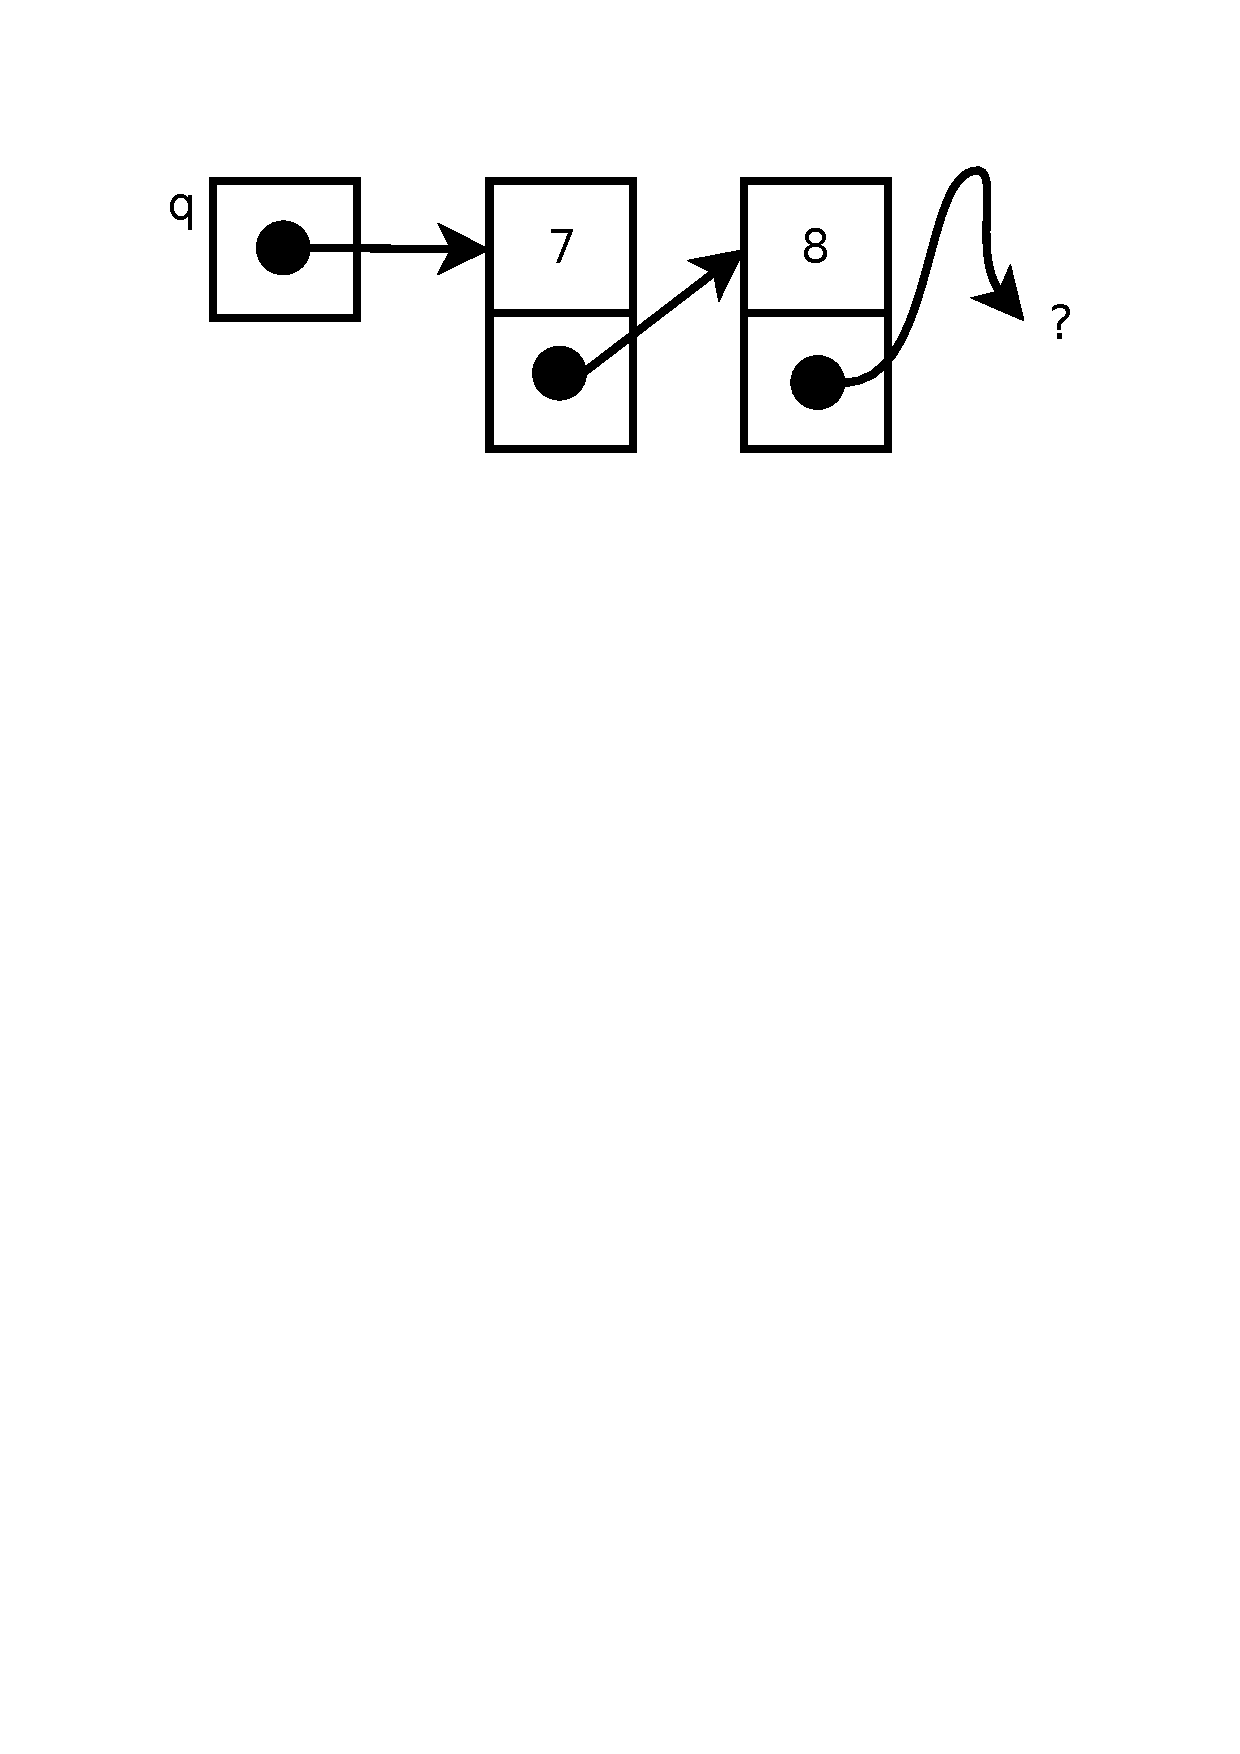
\includegraphics[trim={2.0cm 20.0cm 2.0cm 1.0cm},clip]{queue}}
\end{center}

\emph{Important advice:  drawing pictures is very helpful here. If you are unsure about any code involving pointers, draw a picture.}

If we were sure that the queue had at least 4 items in it, we could write \lstinline!q->next->next->next->data!.
This brings up an important point.
It is critical that the end of linked data structures be properly indicated.
In this case setting the \texttt{next} member to \texttt{0}.
If this ``invariant'' is preserved, you could output all the items in a queue like this:
\begin{codeinline}
struct queue* t=q;
while (t!=0) {
    printf("%d\n", t->data);
    t=t->next;
}
\end{codeinline}

\emph{instruction: stop and make sure you understand exactly what the above does.}

There a number of different visual conventions for indicating a null pointer and it probably doesn't 
matter too much which one you use provided you are consistant. 
Here are some examples:

\begin{center}
\scalebox{0.5}{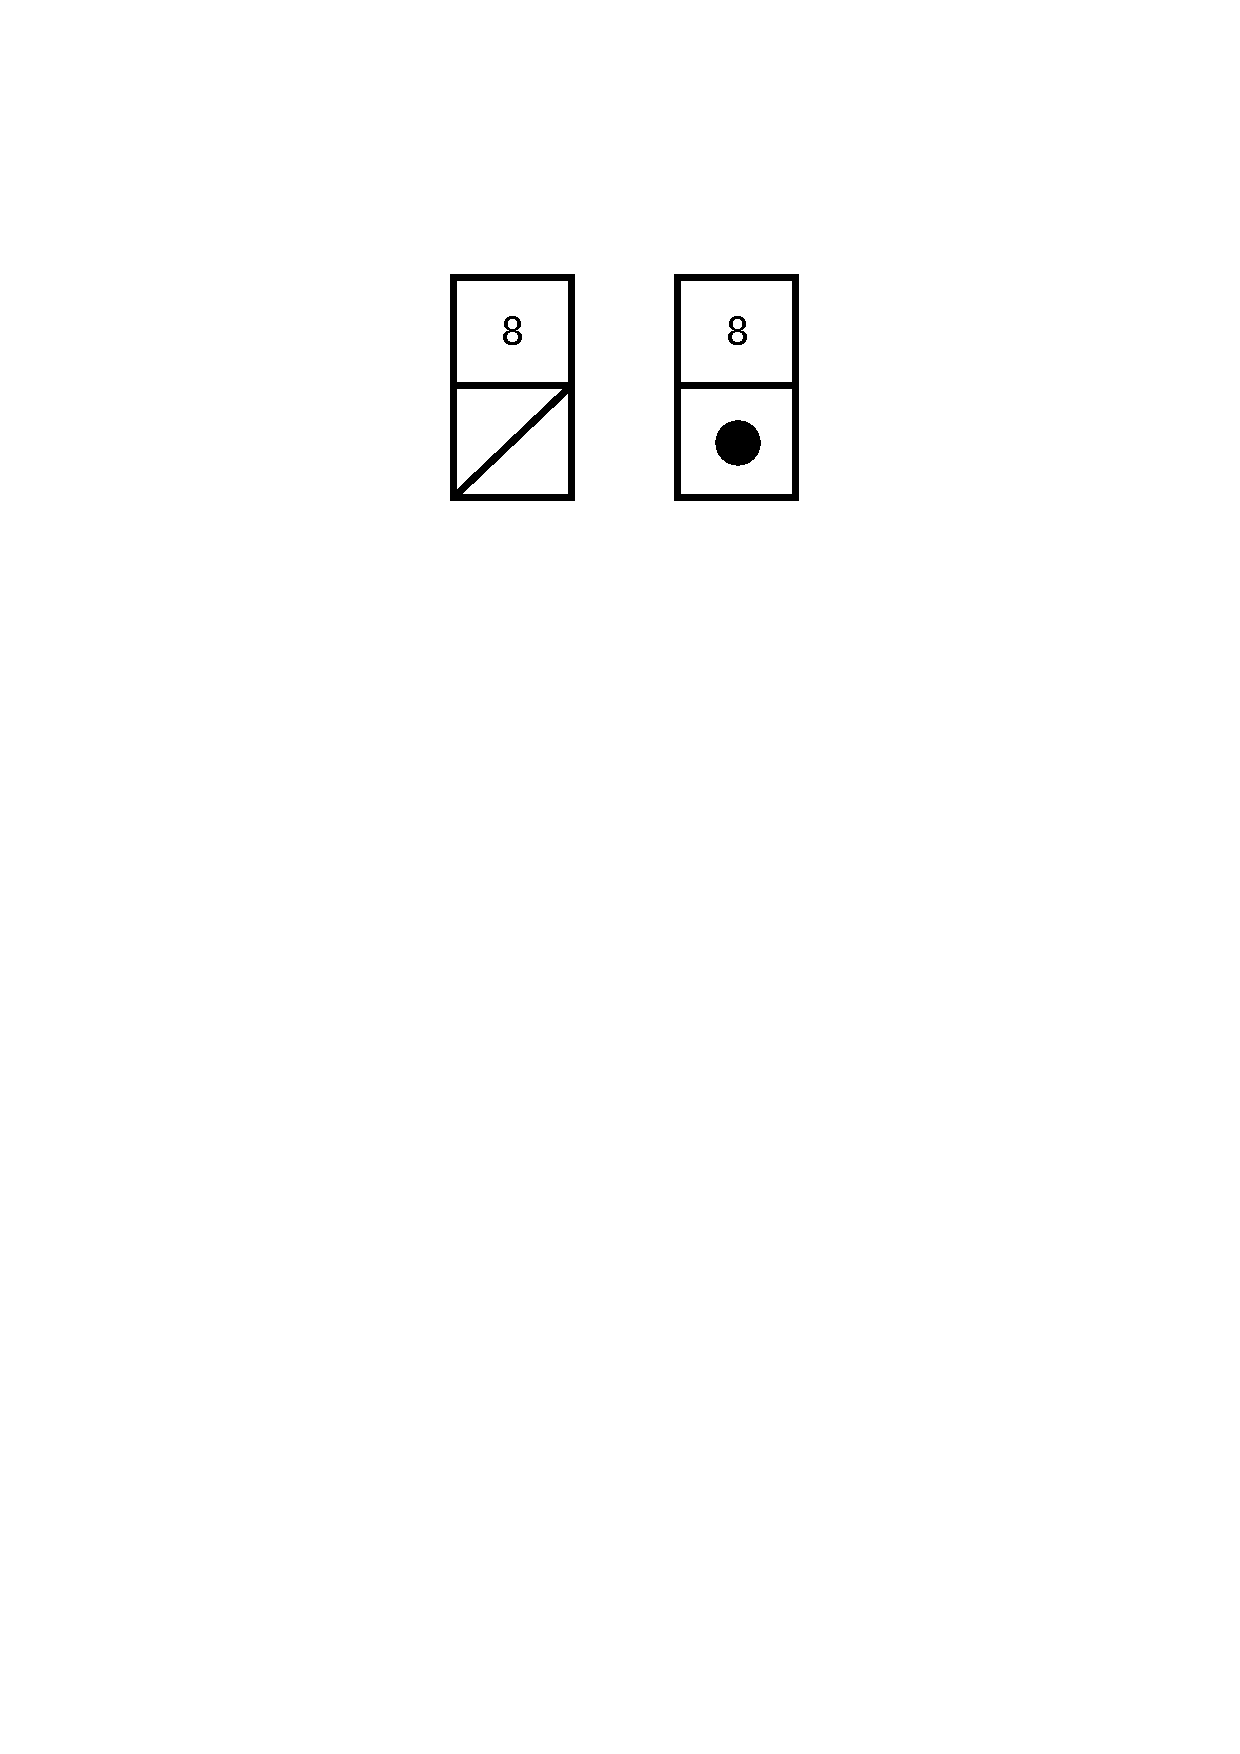
\includegraphics[trim={2.0cm 20.0cm 2.0cm 4.0cm},clip]{nullptr}}
\end{center}



Now we'll add a nicer interface around the queue\_node to make it easier to use.

\begin{codeinline}
struct queue {
    struct queue_node* head;
    struct queue_node* tail;
};
\end{codeinline}

As an optional feature, we could use a \texttt{typedef} to shorten the name.
\begin{codeinline}
typedef struct queue queue;
\end{codeinline}

Since the queue involves memory allocation, we should have setup and teardown/cleanup functions.
\begin{codeinline}
void init_queue(queue* q);
void free_queue(queue* q);
\end{codeinline}
The \lstinline!init_queue()! function assumes that you have already has a queue struct but that it has not been initialised yet.
\begin{codeinline}
queue q;
init_queue(&q);
\end{codeinline}

As an alternative, you could have a function which allocates a queue as well: \lstinline!queue* alloc_queue()!.
Other functions we will need are:
\begin{codeinline}
void add_queue(queue* q, int i);
int get_queue(queue* q);
\end{codeinline}

Notice that this interface doesn't mention malloc even though we know it will be using it.
Let's provide the implementation for these functions.
\begin{codeblock}
void init_queue(queue* q) {
    q->head=0;
    q->tail=0;
}

void free_queue(queue* q) {
    struct queue_node* t=q->head;
    while (t!=0) {
	    // we need this so we can free it
        struct queue_node* temp=t; // after t has moved on
        t=t->next;		
        free(temp);
    }
}
\end{codeblock}

We will add new elements to the end (tail) of the queue and remove items from the front (head) of the queue.
\begin{codeblock}
void add_queue(queue* q, int d) {
      // don't forget the special case of an empty queue
    if (q->head==0) {	
        q->tail=q->head=malloc(sizeof(struct queue_node));
        q->head->next=0;
    } else {
	struct queue_node* n=malloc(
	    sizeof(struct queue_node));
	n->next=0;
	q->tail->next=n
	q->tail=n;
    }
    q->tail->dat=d;
}

int get_queue(queue* q) {
	// check for empty queue first
    if (q->head==0) {
	  // what to do here??
	return 0;
    }
    int result=head->data;
    struct queue_node* temp=q->head;
    q->head=q->head->next;
    free(temp);
      // now we need to check if we have emptied the queue
    if (q->head==0) {
        q->tail=0;
    }
    return result;
}

\end{codeblock}









\section*{Queue summary}
\begin{itemize}
 \item Use structs to carry around all the related variables for a type.
 \item Write setup and cleanup functions for your struct first.
 \item Watch out for special cases.
\end{itemize}


\chapter*{Glossary}

\begin{description}
 \item[\hypertarget{defn:argument}{Argument}] a value supplied to a function to tell it what it should be doing.
 For example (if \texttt{sqrt} computes square roots, then in \lstinline{sqrt(36)}, $36$ is an argument but the same function
 could be called later with a different argument.
 
 Note that arguments are distinct from the names given to the variables the arguments are stored in inside the function (see \hyperlink{defn:parameter}{Parameters}).
 \item[\hypertarget{defn:array}{Array}] A variable, which contains multiple values intead of just one. 
 Individual values are accessed by their \texttt{index} within the array.
 In most C derived langages this is indicated with brackets.
 eg:
    \lstinline!scores[17]!
    
 In C, all the values have the same type and the size of the array is fixed 
 when it is created.
 
 \item[\hypertarget{defn:parameter}{Parameter}] A piece of information which a function needs in order to do it's job.
 For example: the function for computing a square root could be declared as:
 \lstinline!double sqrt(double x)!.
 In order to work, the function needs to know which number it should be taking the square root of.
 In this case, that information will be stored in a variable called \texttt{x}.
 Note that parameters are distinct from \hyperlink{defn:argument}{Argument}s which are the values given in a specific call.
 
 \item[\hypertarget{defn:string}{String}] A sequence of characters which can be manipulated as a unit.
 In C dervied languages, they are usually written in code surrounded by double quotes\footnote{The widley known exception 
 is python, where single or double quotes can be used for strings.}.
 eg:
 \lstinline!"Welcome to C"!
\end{description}

\appendix

\chapter{How to attack a spec}

% Here is where we discuss how to think about programming tasks.
% How do you decide what functions you need?
% How do you break down a task

The following is a specification for a programming task.
You are not expected to actually code this.
The goal instead is to look at how it could be broken into managable pieces 
for a sane development strategy.

Read through the following assignment spec.
In Section~\ref{sec:breakdown}, we'll discuss it.

\section{Introduction}
Your task is to write an \emph{ANSI-C} program (called match) which
allows the user to play a game.

match will display a grid of cells, each containing a symbol.
The user will nominate a cell (by entering its coordinates).
If the symbol in the cell matches the symbol in
any of the cells directly above, below, left or right, then the selected cell and any of its matching neighbours
will be removed.
This effect is also applied to neighbours of matching neighbours (and so on).
As an example, suppose the grid contents (surrounded by a border) were:

\begin{center}
\begin{verbatim}
+-----+
|ZAAAA|
|ZBBCC|
|ZWaaX|
|XXXXX|
|Zcdef|
+-----+
\end{verbatim}
\end{center}
and the cell \texttt{3 1} was chosen (that is, Row~\texttt{3} and Column~\texttt{1}, with the top left being \texttt{0 0}).
In this case, all of Row~\texttt{3} would be removed as well as the last value on Row~\texttt{2}.

\pagebreak
\begin{center}
\begin{verbatim}
+-----+
|ZAAAA|
|ZBBCC|
|ZWaa.|
|.....|
|Zcdef|
+-----+
\end{verbatim}
\end{center}

If a move leaves a gap in the middle of a column, the symbols above it will be moved down to fill the
the gap.

\begin{center}
\begin{verbatim}
+-----+
|.....|
|ZAAA.|
|ZBBCA|
|ZWaaC|
|Zcdef|
+-----+
\end{verbatim}
\end{center}

If \texttt{4 1} was chosen, nothing would happen because the `c' in that cell is not touching any other `c's.
If a removal leaves one or more whole columns empty, any columns to the right of the empty ones, will be
moved over to fill the gap.
For example, if \texttt{1 0} was chosen in the above, the result would be:

\begin{center}
\begin{verbatim}
+-----+
|.....|
|AAA..|
|BBCA.|
|WaaC.|
|cdef.|
+-----+
\end{verbatim}
\end{center}

If the grid looked like:
\begin{center}
\begin{verbatim}
+-----+
|AAAAA|
|ZABAC|
|ZAaAX|
|XAXAX|
|ZAdAf|
+-----+
\end{verbatim}
\end{center}
and \texttt{0 0} was chosen, the result would be:
\begin{center}
\begin{verbatim}
+-----+
|.....|
|ZBC..|
|ZaX..|
|XXX..|
|Zdf..|
+-----+
\end{verbatim}
\end{center}

The game ends when either all the symbols are removed, or there are no more legal moves.


\subsection{Invocation}\label{sec:invoc}
\noindent
When run with no arguments, match should print usage instructions to stderr:\\
\begin{verbatim}
Usage: match height width filename
\end{verbatim}
and exit (see the error table).

\texttt{height} and \texttt{width} must be positive integers greater than 1 and less than \texttt{1,000}.
\texttt{filename} must be a path to a readable file containing a valid grid (see later) with dimensions matching \texttt{height}
and \texttt{width}.
See the error table for what to do if these constraints are not met.

When run with valid arguments, match should read in the map file.
It should then display the grid.
If there are no legal moves, it should exit with the appropriate message; otherwise it should display the prompt:
\begin{verbatim}
>
\end{verbatim}
(note, a space follows the prompt).
The user should then enter either:
\begin{itemize}
 \item the row and column they wish to remove (space separated). eg \texttt{3 2}
 \item \texttt{w} followed immediately by a filename(or path). eg \texttt{whello}
 This will result in the current grid (including the border) being written to a file called ``hello''.
\end{itemize}
If there is no more input from the user, a message should be displayed (see error table) and
the program should exit normally.
If the user enters anything else, the prompt should be displayed again.

After the user has entered a legal (non-w) move, the grid should be updated and displayed again.
If the game is over, display the appropriate message and exit.
If not, display the prompt again and wait for another move.

\subsection{Input file format}
A valid grid file will consist of rows of symbols (and blanks) terminated by newlines (\verb|\n|).
You may use whichever characters you want for grid symbols except the following:
\begin{itemize}
 \item \verb|\0|          --- the null character. This should trigger an error in your program.
 \item \verb|\n|   --- newlines will always be interpretted as the end of a line.
 \item \verb|.| --- a dot indicates a blank. You can include these in your input but the gaps will not be filled until
 a valid move has been completed.
\end{itemize}

\subsection{Errors and messages}\label{sec:errs}
When one of the conditions in the following table happens, the program should print the error message and exit with
the specified status.
All error messages in this program should be sent to \emph{standard error}.
Error conditions should be tested in the order given in the table.
All messages are followed by a newline.

\begin{center}
\begin{tabular}{|p{4cm}|c|p{5.5cm}|}\hline
\textbf{Condition} & \textbf{Exit Status} & \textbf{Message} \\\hline
Program started with incorrect number of arguments & 1 & Usage: match height width filename \\\hline
Invalid grid dimensions & 2 & Invalid grid dimensions \\\hline
Cannot open grid file& 3 & Invalid grid file \\\hline
Error reading grid. Eg: bad chars in input, not enough lines, short lines & 4 & Error reading grid contents \\\hline
\end{tabular}
\end{center}
For a normal exit, the status will be \texttt{0} and no special message is printed.

There are a number of conditions which should cause messages to be displayed but which should not immediately terminate the program.
These messages should also go to standard error.

\begin{center}
\begin{tabular}{|p{5.0cm}|c|p{4cm}|}\hline
\textbf{Condition} & \textbf{Action} & \textbf{Message} \\\hline
Error opening file for saving grid & Prompt again & Can not open file for write \\\hline
Save of grid successful & Prompt again & Save complete \\\hline
End of input while waiting for user input & exit program normally & End of user input \\\hline
\end{tabular}
\end{center}

If after a move, all the symbols have been removed, the program should display ``Complete'' to stdout and exit normally.
If the game has reached a configuration where completion is impossible and there are no more legal moves,
the program will display ``No moves left'' to stdout and exit normally.

\subsection{Compilation}
Your code must compile with command:\\
\texttt{gcc -Wall -ansi -pedantic ass1.c -o match}

\section{Marks}

\subsection{Functionality criteria}

\begin{center}
\begin{itemize}
\item Command args --- correct response to
\begin{itemize}
 \item incorrect number of args
 \item invalid dimensions
 \item invalid grid filename
\end{itemize}
\item Correctly display initial grid and prompt
\item Reject illegal moves on the initial grid
\item Correctly process a single move:
\begin{itemize}
 \item Single removal from top line
 \item Single removal of whole rightmost column
 \item Single removal covering multiple rows/columns
\end{itemize}
\item Detect no more legal moves
\item Correctly save grid
\item Play complete games with multiple removals
\end{itemize}
\end{center}

\hrule
\section{Comments}\label{sec:breakdown}

Reading the spec we can see some points:
\begin{enumerate}
 \item There is a grid which can store letters.
 \item We don't know how big the grid needs to be until the program starts running (so no fixed sized variables).
 \begin{itemize}
  \item The grid does not change size once the game starts though.
 \end{itemize}
 \item There are rules about removing letters from the grid
 \item There is something about files and file formats
\item There are instructions about command line arguments.
 \item There are instructions about error conditions and what to do when they occur.
 \item There is something about how it should compile. \emph{Do not ignore instructions about the intended target platform. 
 If it does not work on the client's machine, it does not work\footnote{unless the client has a broken environment, but that
 is a separate issue.}.}
 \item Finally there are some sort of criteria.
\end{enumerate}

So where to start?
It seems like taking things out of the grid seems to be important so should we start there?
Probably not.
When working on code, you should be thinking about how you are going to make sure that what you have written is correct.
That is, ``how are you going to test that it complies with the spec?''
Do not fall for the idea that you can just test everything at the end and it will be less work\footnote{This is almost always wrong.}.
The more code you need to search, the harder finding bugs will be.

A better approach is to try to look for smaller chunks of functionality.
That you can write \emph{and test} without needing lots of other code you don't have yet.
When you have completed (and tested) a new chunk of functionality, record that version somewhere (eg in version control)
and then move on.

For example, look at the command line argument checking.
In Section~\ref{sec:invoc} it says that you need to display a message when the program is run with no arguments.
This is easy to write and check:
\begin{itemize}
 \item Run with no arguments and check message.
 \item Run with arguments and no message.
\end{itemize}

Section~\ref{sec:errs} describes some extra errors you need to check to do with command line arguments.
Some have to do with processing the contents of a file, so that might need to wait, but the rest of them
should be reasonable.
Again, test each possibility and save that version.
The reason for storing your code after each bit works is that if you break it later\footnote{This raises
another point. Just because something worked before doesn't necessarily mean it still does.
You will want to recheck earlier tests from time to time as well. This is where
automated testing (sometimes mistakenly called unit testing) can be useful.} (adding more features, you have a 
working version you can go back to).

Now you should have some code you can rely on (and you can easily specify different sizes when testing other parts later).

What to do next may be a bit less obvious.
You could try the file reading code (checking for errors) but you don't have anywhere to put any grid information once you've
read it.
In fact, the next thing to do would probably be the representation of the grid but how to test it?
So you would need to work out how to to store the grid \emph{and} how to display it.
Start with creating and displaying a blank grid.
Then try modifying the grid in code and displaying again to see if things appear in the correct place.
This last point, can only be a temporary modification since a working program would not do this, so remove it once you 
are sure it works\footnote{Another strategy you can employ is to have one or more files which have your functions in them and then
use another file which has test functions in it and call the normal functions from there.}.

Following from there you have a number of options.
Removal of letters? Saving? Loading? Game over detection?
The first two are possible, but you would need to add test code to create various board states to test with, so being able 
to have your testing states in files and pulling them in with load would seem to be easier.

When it comes to dealing with removing letters, rather than trying to solve the whole thing in one go.
Try to identify simple subcases, eg an entire column is removed and build up from there.


\end{document}
